%%%%%%%%%%%%%%%%%%%%%%%%%%%%%%%%%%%%%%%%%
% Beamer Presentation
% LaTeX Template
% Version 1.0 (10/11/12)
%
% This template has been downloaded from:
% http://www.LaTeXTemplates.com
%
% License:
% CC BY-NC-SA 3.0 (http://creativecommons.org/licenses/by-nc-sa/3.0/)
%
%%%%%%%%%%%%%%%%%%%%%%%%%%%%%%%%%%%%%%%%%

%----------------------------------------------------------------------------------------
%	PACKAGES AND THEMES
%----------------------------------------------------------------------------------------

\documentclass{beamer}

\mode<presentation> {

% The Beamer class comes with a number of default slide themes
% which change the colors and layouts of slides. Below this is a list
% of all the themes, uncomment each in turn to see what they look like.

%\usetheme{default}
%\usetheme{AnnArbor}
%\usetheme{Antibes}
%\usetheme{Bergen}
%\usetheme{Berkeley}
%\usetheme{Berlin}
%\usetheme{Boadilla}
%\usetheme{CambridgeUS}
%\usetheme{Copenhagen}
%\usetheme{Darmstadt}
%\usetheme{Dresden}
%\usetheme{Frankfurt}
%\usetheme{Goettingen}
%\usetheme{Hannover}
%\usetheme{Ilmenau}
%\usetheme{JuanLesPins}
%\usetheme{Luebeck}
\usetheme{Madrid}
%\usetheme{Malmoe}
%\usetheme{Marburg}
%\usetheme{Montpellier}
%\usetheme{PaloAlto}
%\usetheme{Pittsburgh}
%\usetheme{Rochester}
%\usetheme{Singapore}
%\usetheme{Szeged}
%\usetheme{Warsaw}

% As well as themes, the Beamer class has a number of color themes
% for any slide theme. Uncomment each of these in turn to see how it
% changes the colors of your current slide theme.

%\usecolortheme{albatross}
%\usecolortheme{beaver}
%\usecolortheme{beetle}
%\usecolortheme{crane}
%\usecolortheme{dolphin}
%\usecolortheme{dove}
%\usecolortheme{fly}
%\usecolortheme{lily}
%\usecolortheme{orchid}
%\usecolortheme{rose}
%\usecolortheme{seagull}
%\usecolortheme{seahorse}
%\usecolortheme{whale}
%\usecolortheme{wolverine}

%\setbeamertemplate{footline} % To remove the footer line in all slides uncomment this line
%\setbeamertemplate{footline}[page number] % To replace the footer line in all slides with a simple slide count uncomment this line

%\setbeamertemplate{navigation symbols}{} % To remove the navigation symbols from the bottom of all slides uncomment this line
}

\usepackage{graphicx} % Allows including images
\usepackage{booktabs} % Allows the use of \toprule, \midrule and \bottomrule in tables
\usepackage{hyperref,tikz}
\usetikzlibrary{arrows,shapes,matrix,positioning}
\usepackage{chemfig,siunitx}
\setcompoundsep{7em}
%----------------------------------------------------------------------------------------
%	TITLE PAGE
%----------------------------------------------------------------------------------------

\title[RNA circuits]{Self-contained RNA inhibition with trans-acting ribozymes} % The short title appears at the bottom of every slide, the full title is only on the title page

\author{Zack Field \& Ryan Tsoi} % Your name
\institute[UC Berkeley] % Your institution as it will appear on the bottom of every slide, may be shorthand to save space
{
University of California \\ % Your institution for the title page
\medskip
\textit{field.zackery@berkeley.edu, ryantsoi@berkeley.edu} % Your email address
}
\date{\today} % Date, can be changed to a custom date

\begin{document}

\begin{frame}
\titlepage % Print the title page as the first slide
\end{frame}

\begin{frame}
\frametitle{Overview} % Table of contents slide, comment this block out to remove it
\tableofcontents 
% Throughout your presentation, if you choose to use \section{} 
% and \subsection{} commands, these will automatically be printed 
% on this slide as an overview of your presentation
\end{frame}

%----------------------------------------------------------------------------------------
%	PRESENTATION SLIDES
%----------------------------------------------------------------------------------------

%------------------------------------------------
\section{Introduction} % Sections can be created in order to organize your presentation into discrete blocks, all sections and subsections are automatically printed in the table of contents as an overview of the talk
%------------------------------------------------

\subsection{Genetic Regulation} % A subsection can be created just before a set of slides with a common theme to further break down your presentation into chunks

\begin{frame}
\frametitle{Promise of Synthetic Biology}

Complexity of eukaryotes $\not\approx$ \# of protein coding genes

\begin{tabular}{l | l | l}
\hline
Oryza sativa (rice)& 470 million & 51,00\\
Gallus gallus (chicken)& 1 billion& 20,000-23,00\\ 
Canis familiaris (dog)& 2.4 billion& 19,00 \\
Mus musculus (mouse)& 2.5 billion& 30,00 \\
Homo sapiens & 2.9 billion& 20,000-25,000\\
\hline
\end{tabular}

\bigskip
The root of complexity is believed to be the regulation of these genes.

However, the creation of novel protein regulatory elements is too difficult.

Re-writers RNA-world may be the key to getting a handle on regulation.           
\end{frame}

%------------------------------------------------

\subsection{Motivation}

\begin{frame}
\frametitle{Motivation}

Toggle switch and repressilator in 2000 (images).
 
\begin{figure}[ht]
  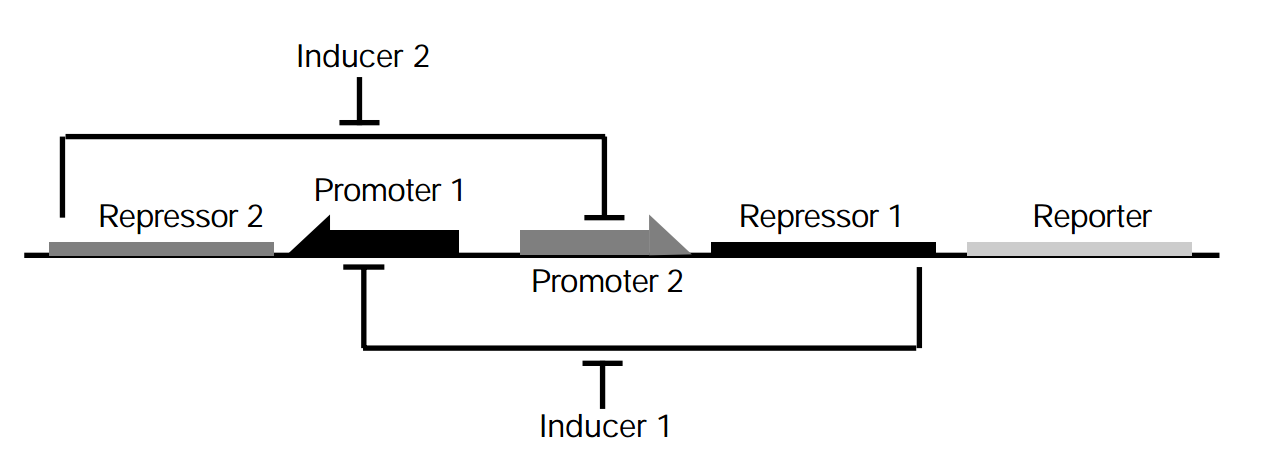
\includegraphics[width=0.5\textwidth]{DNA_toggle.png}
  \hfill
  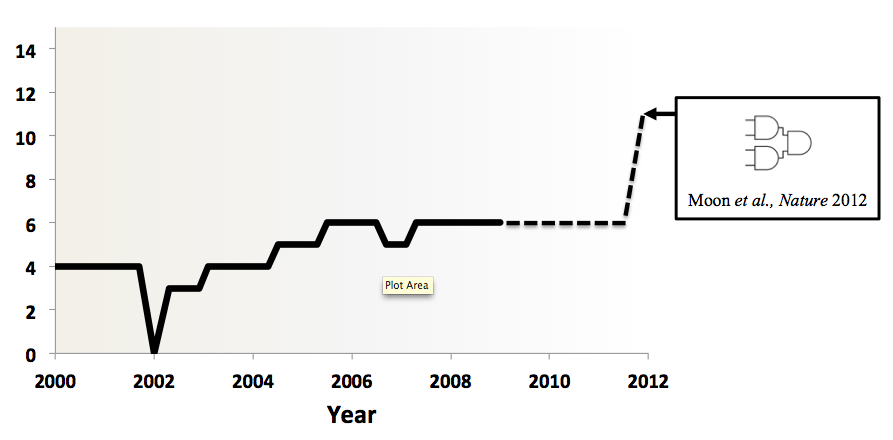
\includegraphics[width=0.5\textwidth]{circuit_complexity.png}
\end{figure}

\begin{figure}[ht]
  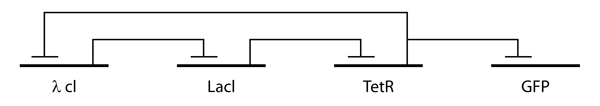
\includegraphics[scale=0.4]{repressilator.png}
\end{figure}
\end{frame}

\begin{frame}
%\frametitle{Motivation}
Exponential decrease in the cost of enabling technologies should result 
in exponential growth of circuit complexity.


  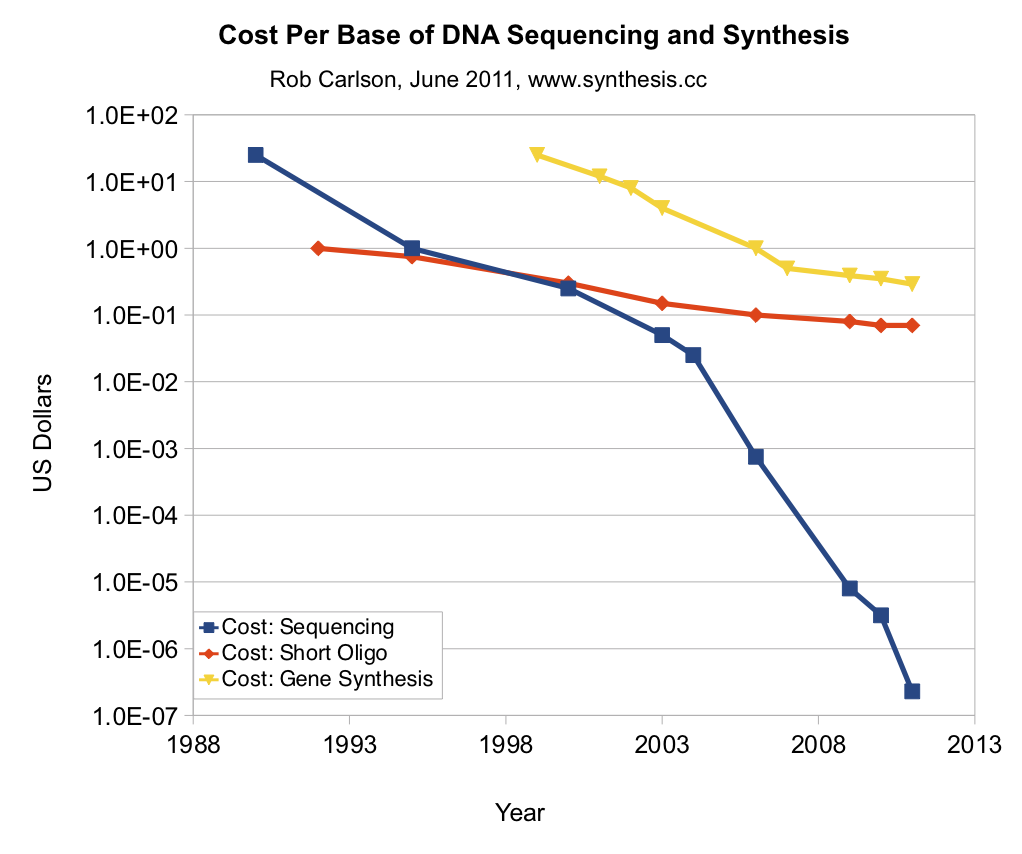
\includegraphics[scale=0.5]{cost_per_base.png}
  
\end{frame}

\begin{frame}
\begin{block}{Pitfalls in current promoter-repressor pair design}
  \begin{itemize}
    \item Orthogonal  - Limited number of repressors (until very recently)
    \item Predictable - Gene circuit evolves away
    \item Safe        - shRNA toxicity in gene therapy
    \item Reliable    - 40 hour toggle switch breakdown
    \item Designable  - Protein structure prediction too difficult
    \item Cooperativity - Unpredictable behavior when juxtaposed
  \end{itemize}
\end{block}

\end{frame}

%------------------------------------------------

\subsection{Types of riboregulation}
\begin{frame}
\frametitle{Types of riboregulation}

Why shRNA sucks, because of cleaving mechanism. But this can
be avoided.

Self-contained action. removes some dependencies.
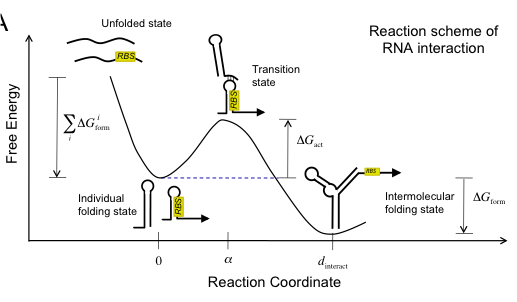
\includegraphics[scale=1]{energy_riboregulation.png}

\end{frame}

%------------------------------------------------
\section{Specific riboregulation decision}
\subsection{Choice of ribozyme}

\begin{frame}
\frametitle{Choice of trans-acting ribozymes}
Proof of functional completeness

Include reasoning for not having apatamer effected
ribozymes. More difficult to design and predict than
simple oligonucleotide effectors. 

Watson Crick base pairing dominates free energy minimization
\end{frame}

%------------------------------------------------

\subsection{General riboregulation model}
\begin{frame}
\frametitle{General riboregulation model}
Stochastic model - Gillespie algorithm

The probability 

Rate of trans cleaving
\end{frame}

%------------------------------------------------

%\subsection{Toggle switch model DNA-based}
%\begin{frame}
%\frametitle{Toggle switch model DNA-based}
%
%\end{frame}

%------------------------------------------------

\subsection{Toggle switch model riboregulation}
\begin{frame}
  \frametitle{Toggle switch model riboregulation}

No possible bistable point. First limitation.

\begin{columns}[T]
    \begin{column}{0.5\textwidth}
      \centering
       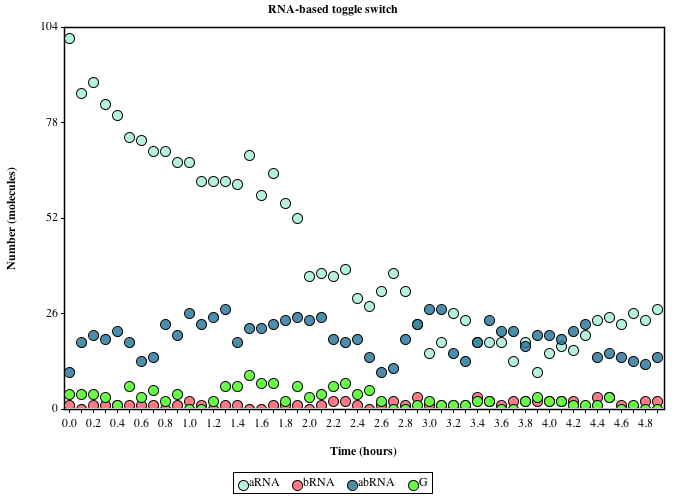
\includegraphics[scale=0.3]{RNA_based_toggle_timecourse.png}
    \end{column}
    \begin{column}{0.5\textwidth}
      \centering
      \scalebox{0.5}{
      \schemestart
      $a_{DNA}$%\phantom{I}
      \arrow{->[$k_{a_{tc}}$]}
      $a_{RNA}$\phantom{}
      \arrow{<=>[*0$k_{a_{on}}$][*0$k_{a_{off}}$]}[-90]
      $a_{RNA}\cdot b_{RNA}$
      \arrow{<=>[*0$k_{b_{on}}$][*0$k_{b_{off}}$]}[-90]
      $b_{RNA}$
      \arrow{<-[$k_{b_{tc}}$]}[180]
      $b_{DNA}$
      \arrow(@c2--){->[$k_{a_{deg}}$]}
      $\emptyset$
      \arrow(@c3--){->[$k_{ab_{deg}}$]}
      $\emptyset$
      \arrow(@c4--){->[$k_{b_{deg}}$]}
      $\emptyset$
      \schemestop    
      }
    \end{column}
  \end{columns}
\end{frame}

%------------------------------------------------

\subsection{Parameter Comparison}
\begin{frame}
\frametitle{Parameter Comparison}


\end{frame}

%------------------------------------------------

\section{Implications and further work}
\begin{frame}
\frametitle{Implications and further work}
If these 
\end{frame}

%------------------------------------------------

\subsection{Sources}
\begin{frame}
\frametitle{Souces}

\begin{itemize}
\item Pray, L. A.; \url{http://www.nature.com/scitable/topicpage/eukaryotic-genome-complexity-437}
\item Arkin, A. and Weiss, Ron; Principles of Synthetic Biology Fall 2013; Lecture 3
\item Carlson, Rob; DNA cost curves; \url{http://www.synthesis.cc/2011/06/new-cost-curves.html}
\item Stanton, B.C. et. al.; \emph{Genomic Mining of prokaryotic repressors for orthogonal logic gates};
  \url{http://www.nature.com/nchembio/journal/vaop/ncurrent/full/nchembio.1411.html}
\item Martin, J.N., et. al.; Lethal toxicity caused by expression of shRNA in the mouse striatum: implications for therapeutic design;
  \url{http://www.nature.com/gt/journal/v18/n7/full/gt201110a.html}
\item Bongarets; \emph{GFP as a Marker for Conditional Gene Expression in Bacterial Cells}
  \url{http://www.ifr.ac.uk/Safety/molmicro/pubs/bongaerts2002.pdf}
\item Anderson, J.C.; \emph{org.devicecourse Gillespie module}
\item Gillespie, Daniel T. (1977). \emph{Exact Stochastic Simulation of Coupled Chemical Reactions}. The Journal of Physical Chemistry 81 (25): 2340–2361. doi:10.1021/j100540a008.
\end{itemize}

\end{frame}

%------------------------------------------------
\begin{frame}
\frametitle{Blocks of Highlighted Text}


\begin{block}{Block 2}
Pellentesque sed tellus purus. Class aptent taciti sociosqu ad litora torquent per conubia nostra, per inceptos himenaeos. Vestibulum quis magna at risus dictum tempor eu vitae velit.
\end{block}

\begin{block}{Block 3}
Suspendisse tincidunt sagittis gravida. Curabitur condimentum, enim sed venenatis rutrum, ipsum neque consectetur orci, sed blandit justo nisi ac lacus.
\end{block}
\end{frame}

%------------------------------------------------

\begin{frame}
\frametitle{Multiple Columns}
\begin{columns}[c] % The "c" option specifies centered vertical alignment while the "t" option is used for top vertical alignment

\column{.45\textwidth} % Left column and width
\textbf{Heading}
\begin{enumerate}
\item Statement
\item Explanation
\item Example
\end{enumerate}

\column{.5\textwidth} % Right column and width
Lorem ipsum dolor sit amet, consectetur adipiscing elit. Integer lectus nisl, ultricies in feugiat rutrum, porttitor sit amet augue. Aliquam ut tortor mauris. Sed volutpat ante purus, quis accumsan dolor.

\end{columns}
\end{frame}

%------------------------------------------------
\section{Second Section}
%------------------------------------------------

\begin{frame}
\frametitle{Table}
\begin{table}
\begin{tabular}{l l l}
\toprule
\textbf{Treatments} & \textbf{Response 1} & \textbf{Response 2}\\
\midrule
Treatment 1 & 0.0003262 & 0.562 \\
Treatment 2 & 0.0015681 & 0.910 \\
Treatment 3 & 0.0009271 & 0.296 \\
\bottomrule
\end{tabular}
\caption{Table caption}
\end{table}
\end{frame}

%------------------------------------------------

\begin{frame}
\frametitle{Theorem}
\begin{theorem}[Mass--energy equivalence]
$E = mc^2$
\end{theorem}
\end{frame}

%------------------------------------------------

\begin{frame}[fragile] % Need to use the fragile option when verbatim is used in the slide
\frametitle{Verbatim}
\begin{example}[Theorem Slide Code]
\begin{verbatim}



\begin{frame}
\frametitle{Theorem}
\begin{theorem}[Mass--energy equivalence]
$E = mc^2$
\end{theorem}
\end{frame}\end{verbatim}
\end{example}
\end{frame}

%------------------------------------------------

\begin{frame}
\frametitle{Figure}
Uncomment the code on this slide to include your own image from the same directory as the template .TeX file.
%\begin{figure}
%\includegraphics[width=0.8\linewidth]{test}
%\end{figure}
\end{frame}

%------------------------------------------------

\begin{frame}[fragile] % Need to use the fragile option when verbatim is used in the slide
\frametitle{Citation}
An example of the \verb|\cite| command to cite within the presentation:\\~

This statement requires citation \cite{p1}.
\end{frame}

%------------------------------------------------

\begin{frame}
\frametitle{References}
\footnotesize{
\begin{thebibliography}{99} % Beamer does not support BibTeX so references must be inserted manually as below
\bibitem[Smith, 2012]{p1} John Smith (2012)
\newblock Title of the publication
\newblock \emph{Journal Name} 12(3), 45 -- 678.
\end{thebibliography}
}
\end{frame}

%------------------------------------------------

\begin{frame}
\Huge{\centerline{The End}}
\end{frame}

%----------------------------------------------------------------------------------------

\end{document} 